\documentclass[10pt]{article}
\usepackage[polish]{babel}
\usepackage[utf8]{inputenc}
\usepackage[T1]{fontenc}
\usepackage{amsmath}
\usepackage{amsfonts}
\usepackage{amssymb}
\usepackage[version=4]{mhchem}
\usepackage{stmaryrd}
\usepackage{graphicx}
\usepackage[export]{adjustbox}
\graphicspath{ {./images/} }

\title{GIMNAZJUM }

\author{}
\date{}


\begin{document}
\maketitle
\begin{enumerate}
  \item W czworokącie wypukłym środki boków połączono z wierzchołkami tak, jak na rysunku. Udowodnij, że pole czerwonego czworokąta jest równe sumie pól niebieskich trójkątów.
  \item Udowodnij, że \(\underbrace{22 \ldots 2}_{n}+\underbrace{33 \ldots 3^{2}}_{n}=\underbrace{11 \ldots 1}_{2 n}\)\\
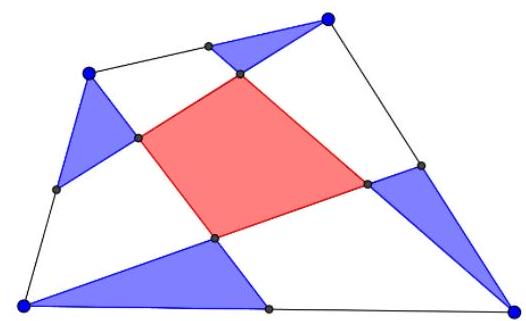
\includegraphics[max width=\textwidth, center]{2024_11_21_a94bec3b7a053690247eg-1}
  \item Trójkąt równoboczny ABC wpisano w okrag i na łuku AB obrano taki punkt P, że odcinek PC przecina bok AB w punkcie Q. Udowodnij, że
\end{enumerate}

\[
\frac{1}{P A}+\frac{1}{P B}=\frac{1}{P Q}
\]

\section*{LICEUM}
\begin{enumerate}
  \item Jacek zrobił sobie filiżankę kawy. Wypił pół filiżanki i dolał mleka do pełna. Czynność tę powtórzył kilka razy, za każdym razem wypijając dwa razy mniej niż poprzednio. Na końcu wypił wszystko do dna. Czego wypił więcej: kawy czy mleka?
  \item W tablicy mnożenia wyróżniono tzw. gnomony (zob. rysunek). Udowodnij, że sumy liczb w gnomonach są sześcianami kolejnych liczb naturalnych.
  \item Trójkąt równoboczny \(A B C\) wpisano w okrąg i na łuku \(A B\) obrano taki punkt P, że odcinek PC przecina bok AB w punkcie Q. Udowodnij, że
\end{enumerate}

\[
\frac{1}{P A}+\frac{1}{P B}=\frac{1}{P Q}
\]

\begin{center}
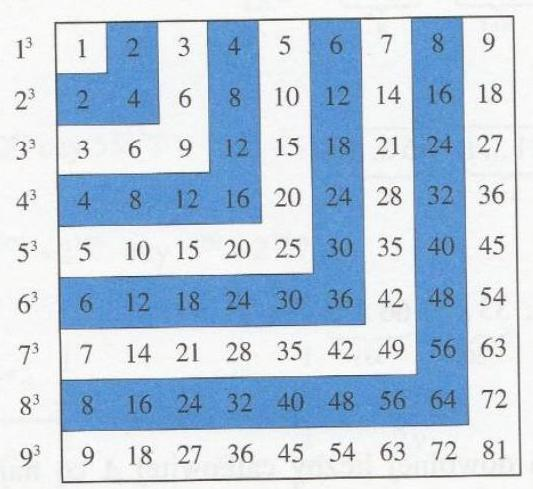
\includegraphics[max width=\textwidth]{2024_11_21_a94bec3b7a053690247eg-1(1)}
\end{center}


\end{document}